Od momentu zapoczątkowania przez Loftiego Zadeha w 1965 roku w artykule ,,Fuzzy
sets'', teoria zbiorów rozmytych odniosła sukcesy w różny sposób w wielu
dyscyplinach. Zastosowania tej teorii można znaleźć na przykład w sztucznej 
inteligencji, medycynie, systemach eksperckich, logice, zarządzaniu, 
rozpoznawaniu wzorców, robotyce i teorii decyzji. Matematyczny rozwój osiągnął 
bardzo wysoki poziom i jest wciąż poszerzany.

Dynamiczny rozwój, początkowo niezauważonej teorii, nastąpił w drugiej połowie 
lat 70-tych rozwiązaniem problemu sterowania piecem do wytwarzania cementu 
wykorzystując logikę rozmytą (Mamdani). Jednak dopiero udane implementacje w 
Japonii zapoczątkowały zainteresowanie na szeroką skalę. Do najgłośniejszych 
sukcesów należy opracowanie układu sterowania metrem w mieście Sendai. Dzięki 
wnioskowaniu rozmytym udało się zmniejszyć czasy opóźnień oraz koszty utrzymania.

W ciągu ostatnich dekad teoria zbiorów rozmytych rozwinęła się w dwóch liniach:
\begin{enumerate}[1)]
  
  \item Jako formalna teoria, która stała się bardziej wyrafinowana i została 
  powiększona o szereg oryginalnych pomysłów i koncepcji, które obejmują obszary 
  klasycznej matematyki (m. in. algebra, teoria grafów, topologia) uogólniając
  je lub ,,rozmywając''.
  
  \item Jako zorientowana na zastosowania ,,rozmyta technologia'', czyli
  narzędzie do między innymi modelowania, rozwiązywania problemów, data mining. 
  W wielu przypadkach udowodniono przewagę zbiorów rozmytych nad istniejącymi 
  metodami, a w innych okazały się one atrakcyjnym dodatkiem do klasycznych 
  rozwiązań.

\end{enumerate}

Poniższy rozdział stanowi krótkie wprowadzenie do teorii zbiorów rozmytych. 
Zostaną również wprowadzone elementy teorii wykorzystywane przy podejmowaniu 
decyzji i niezbędne do zrozumienia dalszej części pracy. Na samym końcu 
przedstawione zostanie kilka przykładów zastosowań logiki rozmytej przy 
grupowym podejmowaniu decyzji.

\section{Elementy teorii zbiorów rozmytych}

\subsection{Podstawowe definicje}
Podstawowym pojęciem opisywanej teorii jest zbiór rozmyty. W klasycznej teorii
zbiorów, z każdym zbiorem $A$ powiązana jest \emph{funkcja charakterystyczna}
$$ \mathcal{X}_A(x) = 
  \left\{ 
	\begin{array}{ll}
	  0, & \quad \textrm{gdy } x \notin A, \\
      1, & \quad \textrm{gdy } x \in A,
  	\end{array} 
  \right. $$  
która dla dowolnego elementu $x$  w uniwersum $\mathcal{X}$ przyjmuje wartość
$1$, jeśli $x$ należy do zbioru $A$, oraz $0$ w przeciwnym przypadku.
Przykładowy wykres funkcji charakterystycznej przedstawiony jest na rysunku
\ref{fig:funkcja_charakterystyczna}. Dla odróżnienia, zbiór rozumiany w sposób
klasyczny będzie nazywany zbiorem ostrym.

\begin{figure}[ht]
  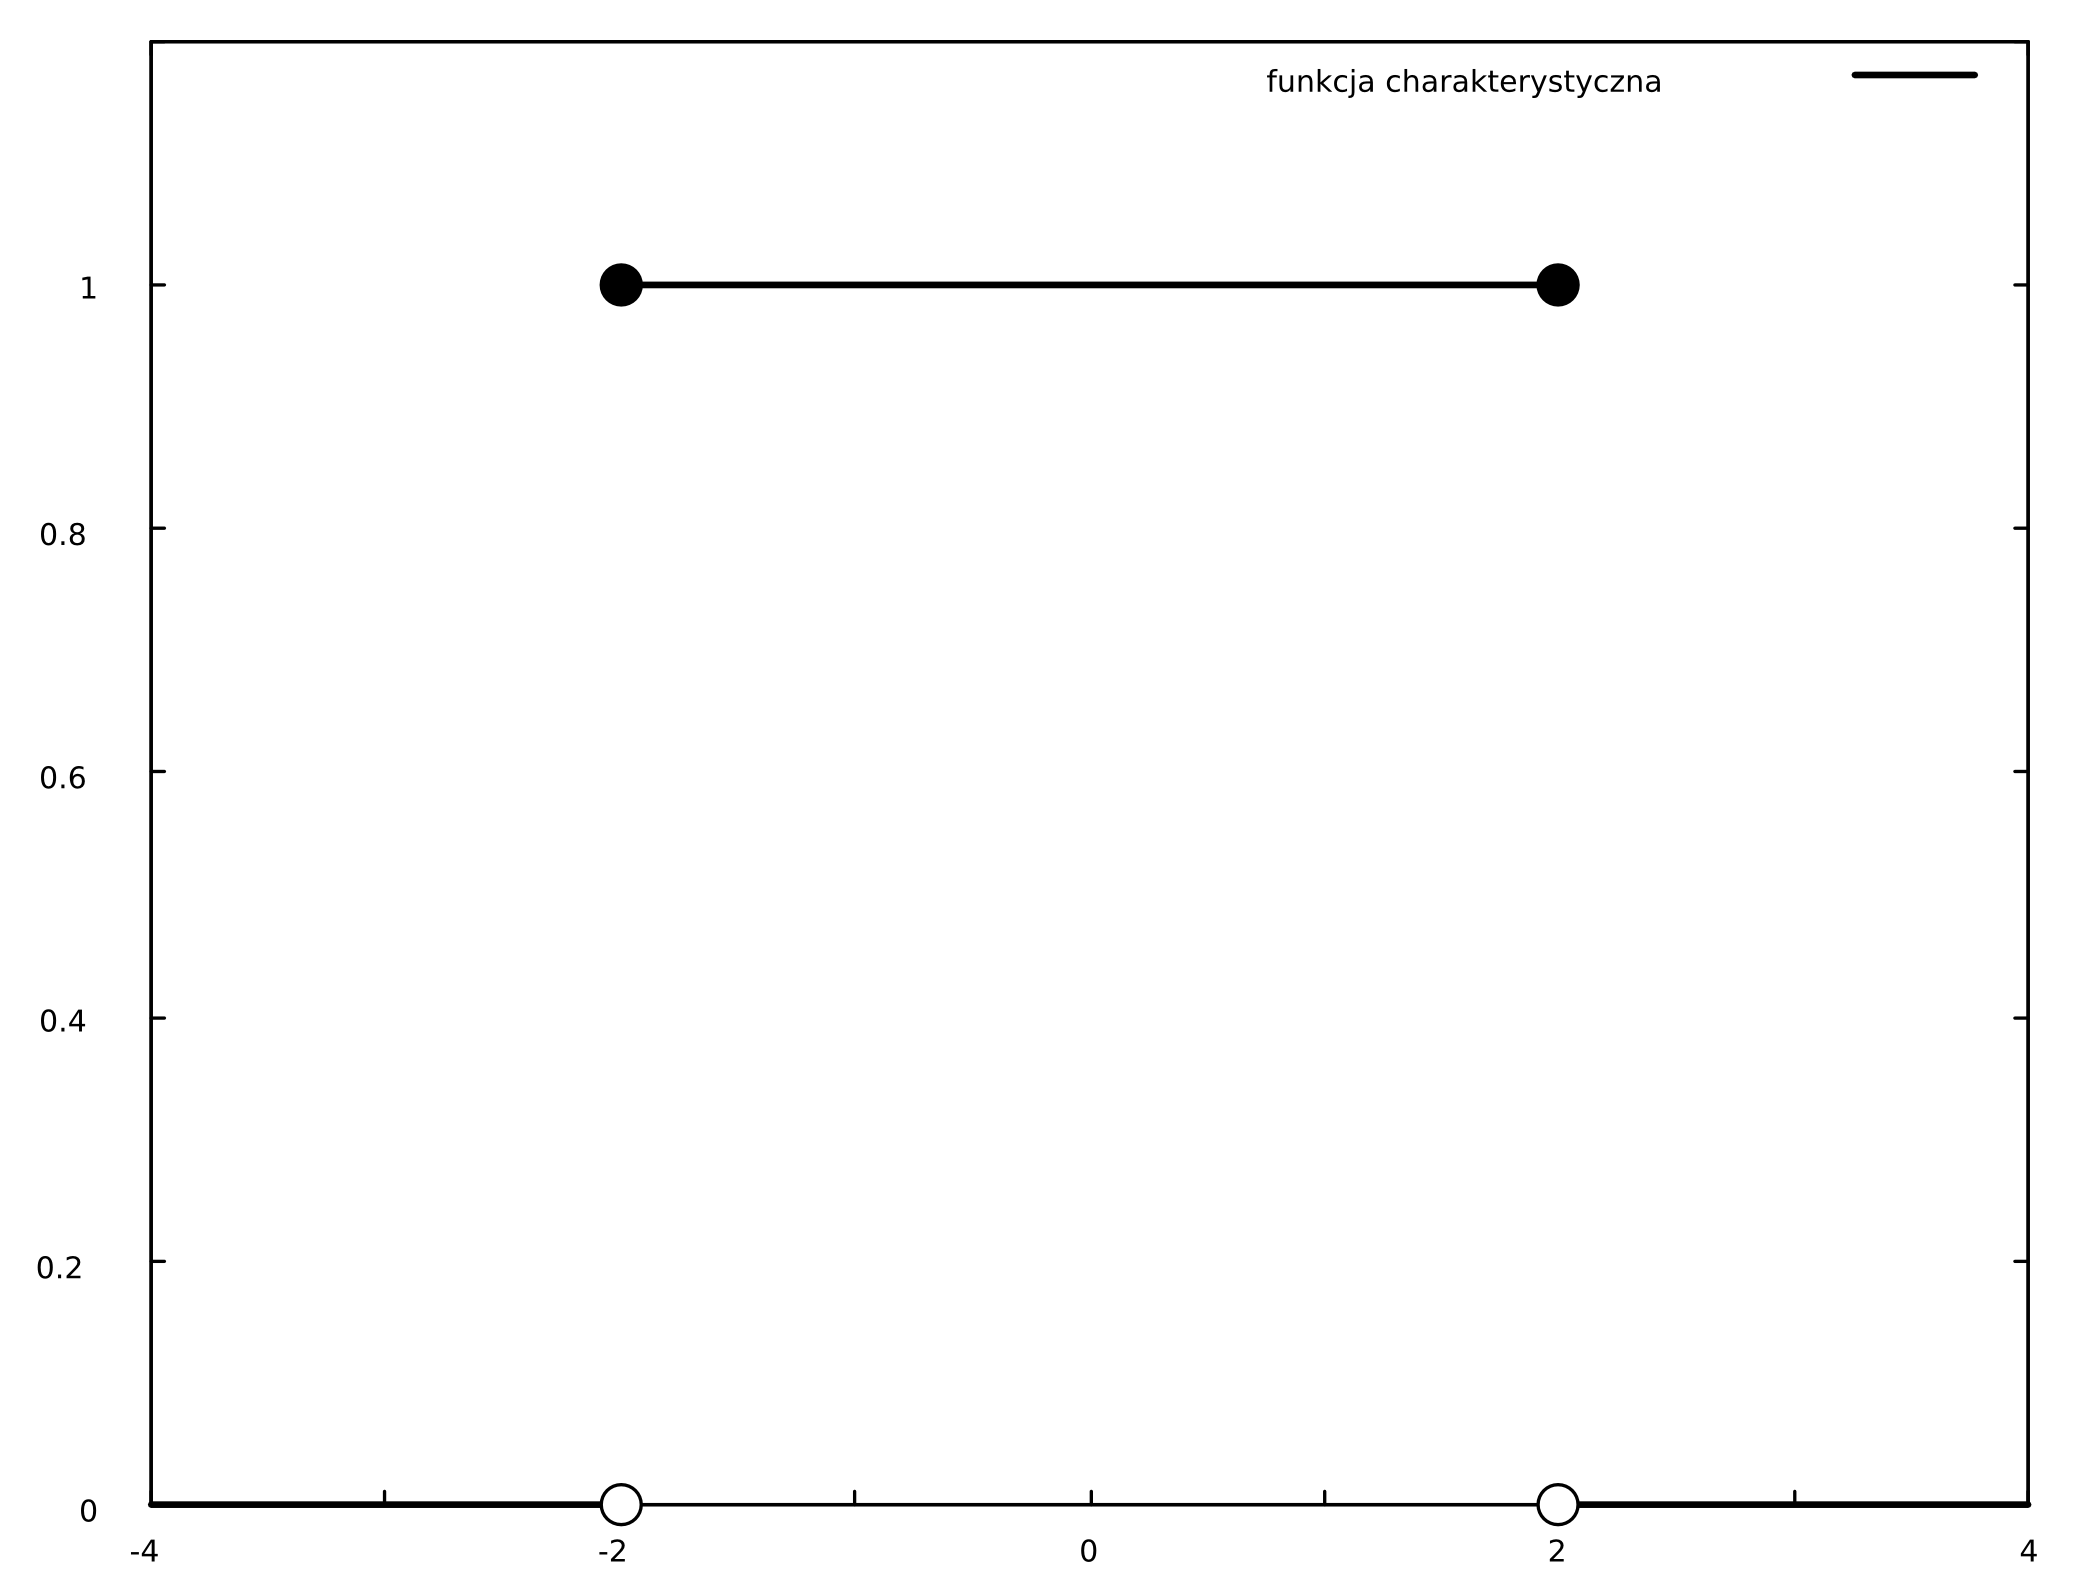
\includegraphics[width=\linewidth]
  	{chapters/fuzzylogic/funkcja_charakterystyczna}
  \caption{Funkcja charakterystyczna dla zbioru $x \in \mathcal{R} : -2 \leq x
  \leq 2 $}
  \label{fig:funkcja_charakterystyczna}
\end{figure}

Powyższa definicja mówi o tym, że jakiś element należy do zbioru lub nie. Jednak
czy w ,,realnym życiu'' zawsze możliwe jest jednoznaczne określenie, że coś
podoba się w $100\%$ lub nie? Albo czy coś jest zawsze w $100\%$ prawdą? W życiu
codziennym na pytanie ,,Czy to miejsce Ci się podoba?'', prócz odpowiedzi
,,tak'' i ,,nie'', bardzo często można usłyszeć: nie do końca, może być, nie
bardzo, jest super, zdecydowanie nie. Każda z tych odpowiedzi opisuje stopień
podobania się. Można się dowiedzieć na przykład, że pytanej osobie dane miejsce
się nie podoba, ale jest skłonna tam pójść.

Pomimo tego, że człowiek doskonale radzi sobie z odpowiedziami typu: ,,bardzo'',
,,około'', ,,mało'', ,,mniej więcej'', itp. to próba ich wyrażenia za pomocą
tradycyjnych zbiorów skazana jest na porażkę. Obserwacja ta była podstawą dla
Zadeha wprowadzenia pojęcia zbioru nieostrego (rozmytego).

\begin{definition}[Zbiór rozmyty]
Jeżeli $\mathcal{X}$ jest kolekcją obiektów to zbiór rozmyty $A$ w przestrzeni
$\mathcal{X}$ określa się jako zbiór (klasyczny) par uporządkowanych
\begin{equation}
A = \{ (x, \mu_A(x)) : x \in \mathcal{X} \},
\end{equation}
gdzie $\mu_A$ jest funkcją przynależności zbioru rozmytego $A$ oraz $\mu_A(x)
\in [0,1]$ nazywany jest stopniem przynależności elementu $x$ do zbioru
rozmytego $A$. Tak zdefiniowany zbiór rozmyty jest tożsamy z funkcją
przynależności, gdyż ta zgodnie z teorią mnogości określona jest jako zbiór par
uporządkowanych.
\end{definition}

Przykładową funkcję przynależności opisującą sformułowanie ,,około zera'' można
zaprezentować jak na rysunku \ref{fig:funkcja_przynaleznosci}.

\begin{figure}[ht]
  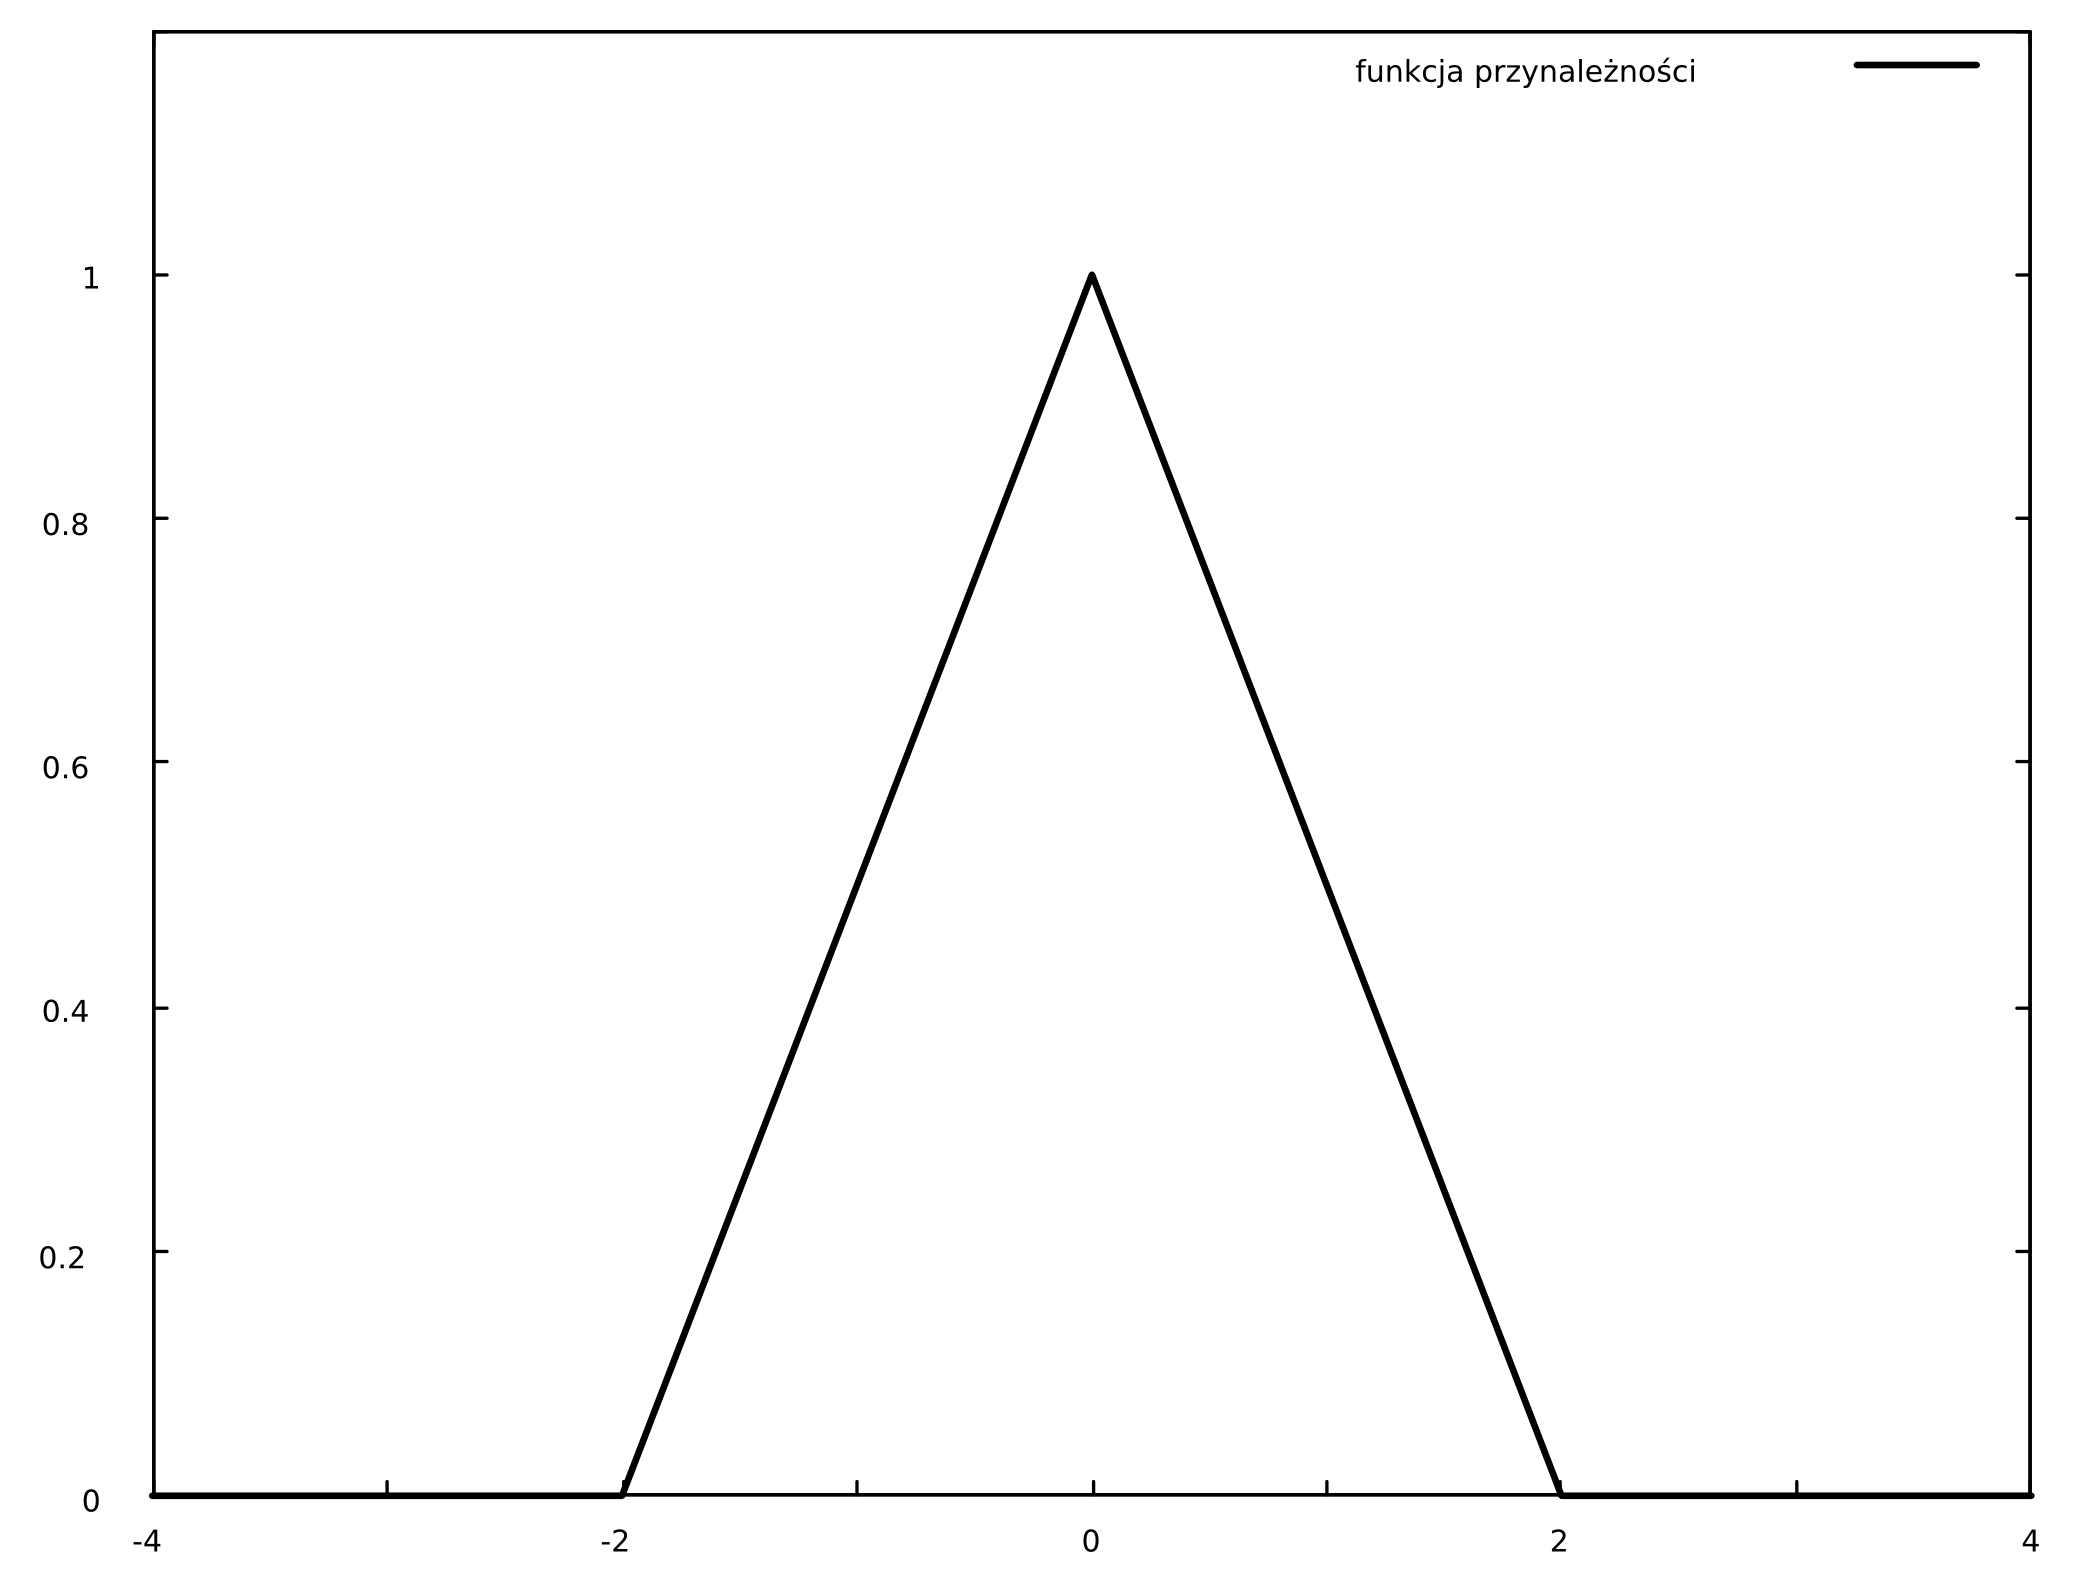
\includegraphics[width=\linewidth]
  	{chapters/fuzzylogic/funkcja_przynaleznosci}
  \caption{Przykładowa funkcja przynależności}
  \label{fig:funkcja_przynaleznosci}
\end{figure}

Ze zbiorami rozmytymi wiąże się kilka przydatnych pojęć przedstawionych poniżej.

\begin{definition}[Nośnik zbioru] Niech $A : X \rightarrow [0,1].$ Zbiór:
\begin{equation}
  \mathrm{supp}(A) = \{ x \in \mathcal{X} : A(x) > 0 \}.
\end{equation}
nazywamy \emph{nośnikiem} (ang. support) zbioru nieostrego.
Nośnik zbioru to inaczej zbiór tych elementów $x$, które mają znaczenie dla $A$.  
\end{definition}

\begin{definition}
Niech $A : X \rightarrow [0,1]$.
\begin{itemize}
  \item \emph{t-przekrojem} i \emph{jądrem} $A$ nazywa się odpowiednio zbiory
  \newline $A_t = \{ x \in X : A(x) \geq t \}$ i $ker(A) = A_1$.
  \item Mówimy, że $A$ jest \emph{skończony}, gdy $supp(A)$ jest zbiorem
  skończonym, a w przeciwnym przypadku $A$ nazywamy \emph{nieskończonym} zbiorem
  nieostrym.
  \item Jeżeli $ker(A) \neq \emptyset,$ mówimy, że $A$ jest \emph{normalny}, a w
  przeciwnym przypadku $A$ nazywamy \emph{podnormalnym} lub \emph{subnormalnym}.
  \item Jeśli $|supp(A)| = 1$, $A$ nazywamy \emph{singletonem}.
\end{itemize}
\end{definition}

\emph{Normalny} zbiór rozmyty nakłada ograniczenie na funkcję przynależności,
które z punktu widzenia teorii jest nieistotne, jednakże w zastosowaniach
praktycznych okazuje się bardzo przydatne. Jeżeli zbiór rozmyty $A$ jest
normalny to wartość funkcji przynależności można interpretować jako procent na
ile dany element $x$ należy do $A$.

Jednym z ważniejszych pojęć zbiorów rozmytych wykorzystywanym przy modelowaniu
podejmowania decyzji jest \emph{zmienna lingwistyczna}. Rozważmy zdania:
\begin{itemize}
  \item[] \emph{Tamto drzewo jest wysokie.}
  \item[] \emph{Ta książka jest droga.}
\end{itemize}

W pierwszym zdaniu atrybutem drzewa jest jego wysokość. Atrybut ten przyjmuje
wartość ,,wysokie''. W drugim przykładzie atrybutem książki jest cena, której
wartość to ,,droga''. Sposób pojmowania tych wartości lingwistycznych może być
różny dla różnych osób, dlatego każda taka wartość charakteryzowana jest zbiorem
rozmytym.

\begin{definition} Zmienną lingwistyczną nazywamy czwórkę $(N,X,T,M_N)$, gdzie

\begin{tabular}{ll}
  $N$ & \qquad nazwa zmiennej (np. \textit{wiek}), \\
  $X$ & \qquad przestrzeń rozważań (np. [0, 125] lat), \\
  $T$ & \qquad zbiór wartości lingwistycznych (terminów) (np. \{młody, średni,
  stary\}), \\
  $M_N$ & \qquad funkcja semantyczna $M_N : T \rightarrow \textrm{zbiór funkcji
  przynależności}$.
\end{tabular}
\end{definition}

Na rysunku \ref{fig:zmienna_lingwistyczna} pokazane są przykładowe funkcje
przynależności dla zbioru termów \{mróz, zimno, chłodno, ciepło, gorąco\}
zmiennej lingwistycznej o nazwie ,,temperatura''. W tym przypadku przestrzenią
rozważań są stopnie Celsjusza od $-25$ do $45$ stopni.

\begin{figure}[ht]
  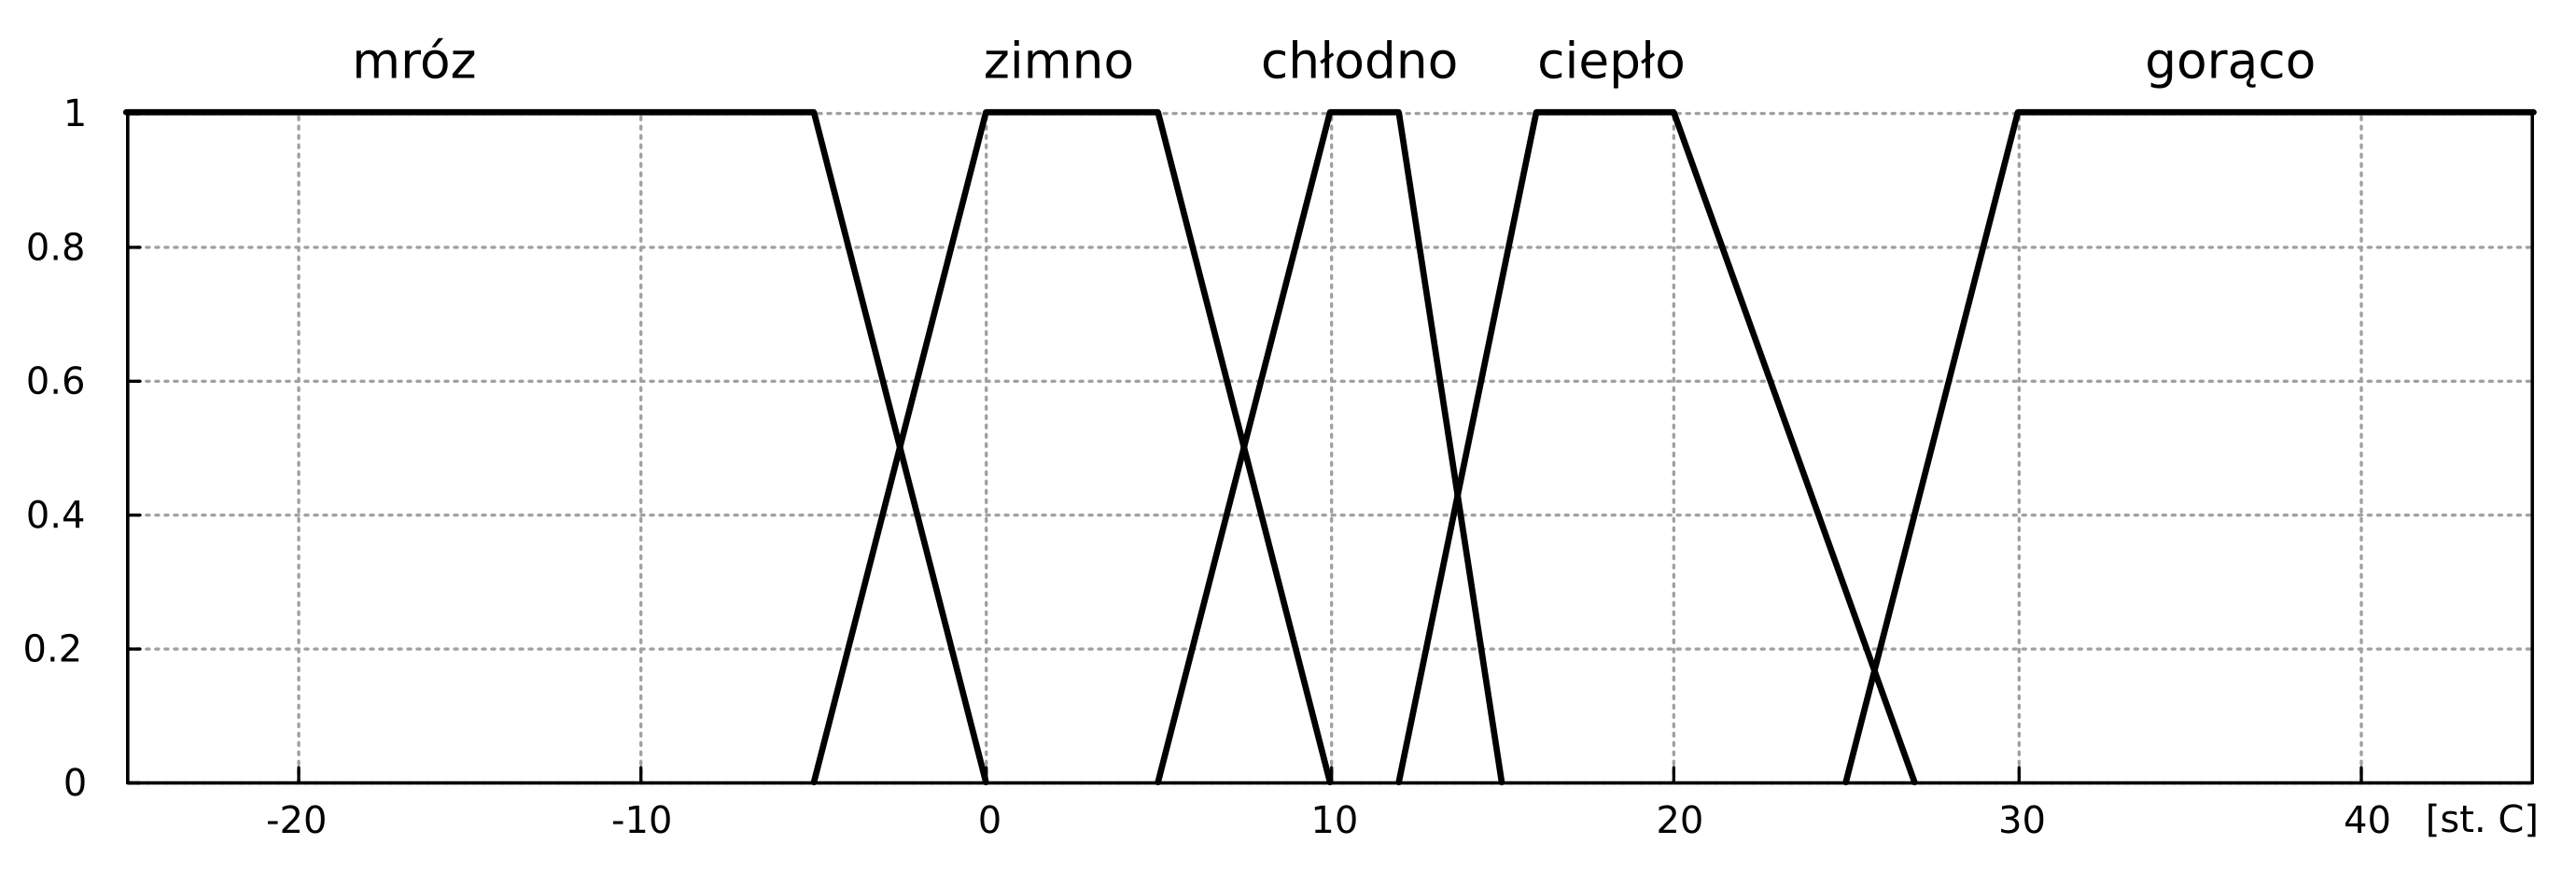
\includegraphics[width=\linewidth]
  	{chapters/fuzzylogic/zmienna_lingwistyczna}
  \caption{Funkcje przynależności dla zmienne lingwistycznej ,,temperatura''}
  \label{fig:zmienna_lingwistyczna}
\end{figure}

\subsection{Operacje na zbiorach rozmytych}
W klasycznej teorii mnogości podstawowe operacje na zbiorach to: dopełnienie,
suma, iloczyn. Nie inaczej jest w przypadku zbiorów rozmytych, ale wszystkie te
operacje można zdefiniować na wiele sposobów.

W swojej pierwszej publikacji, Zadeh zdefiniował podstawowe operacje,
generalizujące operacje dla zbiorów ostrych, w następujący sposób:

\begin{definition}
Dopełnienie zbioru rozmytego $A$ określa się jako zbiór rozmyty, którego funkcja
przynależności dana jest w następujący sposób:
\begin{equation}
\mu_{\neg A}(x) = 1 - \mu_A(x).
\end{equation}
\end{definition}

\begin{definition}
Suma dwóch zbiorów rozmytych $A$ i $B$ określa się jako zbiór rozmyty, którego
funkcja przynależności dana jest w następujący sposób:
\begin{equation}
\mu_{A \cup B}(x) = \max(\mu_A(x), \mu_B(x)).
\end{equation}
\end{definition}

\begin{definition}
Iloczyn dwóch zbiorów rozmytych $A$ i $B$ określa się jako zbiór rozmyty,
którego funkcja przynależności dana jest w następujący sposób:
\begin{equation}
\mu_{A \cap B}(x) = \min(\mu_A(x), \mu_B(x)).
\end{equation}
\end{definition}

Powyższe definicje sumy i przekroju, mimo swej powszechności i intuicyjności,
nie są jedynym sposobem zdefiniowania tych operacji. Rozróżnia się dwie rodziny
funkcji, które dzięki spełnienie pewnych warunków, mogą zastąpić operację
maksimum i minimum w definicjach, odpowiednio, sumy i przekroju zbiorów
rozmytych.

\begin{definition}[t-norma]
Funkcję $t : [0,1] \times [0,1] \rightarrow [0,1]$ nazywamy \emph{normą
triangularną} (krótko: \emph{t-normą}) jeżeli:
\begin{itemize}
  \item funkcja $t$ jest monotoniczna $$a \leq b \Rightarrow t(a,c) \leq
  t(b,c),$$
  \item funkcja $t$ spełnia warunek przemienności $$t(a,b) = t(b,a),$$
  \item funkcja $t$ spełnia warunek łączności $$t(a, t(b,c)) = t(t(a,b),c),$$
  \item funkcja $t$ spełnia warunki brzegowe $$t(a,0)=0 \textrm{ oraz }
  t(a,1)=a,$$
\end{itemize}
gdzie $a, b, c \in [0,1]$.
\end{definition}

Najczęściej spotykane t-normy to:
\begin{itemize}
  \item minimum $$t(a,b) = \min(a,b),$$
  \item iloczyn algebraiczny $$t(a,b) = a \cdot b,$$
  \item t-norma Łukasiewicza $$t(a,b) = \max(0, a+b-1).$$
\end{itemize}

\begin{definition}[t-konorma]
Funkcję $s : [0,1] \times [0,1] \rightarrow [0,1]$ nazywamy \emph{konormą
triangularną} (krótko: \emph{t-konormą}) jeżeli:
\begin{itemize}
  \item funkcja $s$ jest monotoniczna $$a \leq b \Rightarrow s(a,c) \leq
  s(b,c),$$
  \item funkcja $s$ spełnia warunek przemienności $$s(a,b) = s(b,a),$$
  \item funkcja $s$ spełnia warunek łączności $$s(a, s(b,c)) = s(s(a,b),s),$$
  \item funkcja $s$ spełnia warunki brzegowe $$s(a,0)=a \textrm{ oraz }
  s(a,1)=1,$$
\end{itemize}
gdzie $a, b, c \in [0,1]$.
\end{definition}

Najczęściej spotykane t-konormy to:
\begin{itemize}
  \item maksimum $$s(a,b) = \max(a,b),$$
  \item suma probabilistyczna $$s(a,b) = a+b-ab,$$
  \item t-konorma Łukasiewicza $$s(a,b) = \min(a+b,1).$$
\end{itemize}

Ogólne przecięcie i sumę zbiorów rozmytych definiuje się jako:
$$\mu_{A \cap B}(x) = t(\mu_A(x), \mu_B(x)), $$
$$\mu_{A \cup B}(x) = s(\mu_A(x), \mu_B(x)). $$

Przedstawione operacje na zbiorach rozmytych mają własności przemienności,
łączności i rozdzielności, zachodzą również prawa de Morgana. Jest to przydatne
w zastosowaniach praktycznych, jednak w ogólności:

$$A \cap \bar{A} \neq \emptyset \textrm{ i } A \cup \bar{A} \neq \mathcal{X}.$$

\subsection{Relacja rozmyta}
Relacje rozmyte pozwalają sformalizować nieprecyzyjne sformułowania typu ,,$x$
jest prawie równe $y$'' lub ,,$x$ jest znacznie większe od $y$''.

\begin{definition}[Relacja rozmyta]
Relację rozmytą $\mathcal{R}$ między dwoma niepustymi zbiorami ostrymi $X$ i $Y$
nazywamy zbiór rozmyty określony na iloczynie kartezjańskim $X \times Y$, tzn.
$$\mathcal{R} \subseteq X \times Y = \{ (x,y) : x \in X, y \in Y \}.$$
Innymi słowy relacja rozmyta jest zbiorem par
\begin{equation}
\mathcal{R} = \{ ((x,y), \mu_{\mathcal{R}}(x,y)) : x \in X, y \in Y \},
\end{equation}
gdzie $\mu_{\mathcal{R}} : X \times Y \rightarrow [0,1]$ jest funkcją
przynależności. Funkcja ta każdej parze $(x,y)$ przypisuje jej stopień
przynależności $\mu_{\mathcal{R}}(x,y)$, który ma interpretację siły powiązania
między elementami $x$ i $y$.
\end{definition}

\begin{example}
Dana są przestrzenie rozważań $X=\{ x_1,x_2,x_3 \} = \{3,4,5\}$,
$Y=\{y_1,y_2,y_3\} = \{4,5,6\}$ oraz relacja $\mathcal{R} \subseteq X \times Y$
interpretowana jako ,,$y$ jest mniej więcej równe $x$''. Niech relację
$\mathcal{R}$ reprezentuje macierz $[a_{ij}]$, gdzie wartość $a_{ij}$ oznacza
stopień powiązania między elementami $x_i$ i $y_j$:
$$A = 
\begin{pmatrix}
0.8 & 0.6 & 0.4 \\
  1 & 0.8 & 0.6 \\
0.8 &   1 & 0.8
\end{pmatrix}.
$$
Równoważnie można zapisać:
$$
A = 
\left\{ 
	\begin{array}{cl}
	  1, & \quad \textrm{jeżeli } x = y, \\
      0.8, & \quad \textrm{jeżeli } |x - y| = 1, \\
      0.6, & \quad \textrm{jeżeli } |x - y| = 2, \\
      0.4, & \quad \textrm{jeżeli } |x - y| = 3. \\
  	\end{array} 
  \right.
$$
\end{example}

\subsection{Operatory agregacji}
Wiadomo już jak sumować zbiory rozmyte, jak tworzyć ich przecięcie oraz jak
definiuje się relacje. Z punktu widzenia poniższej pracy niezwykle przydatna
jest możliwość agregacji danych. Mając zebrane dane o preferencjach ekspertów w
postaci zbiorów rozmytych, należy zebrać je w jedność w celu zbadania poziomu
konsensusu.

\begin{definition}
\emph{Operatorem agregacji} nazywamy odwzorowanie
$$
Agr: \cup_{n \geq 1} [0,1]^n \rightarrow [0,1],
$$
spełniające następujące warunki:
\begin{itemize}
  \item monotoniczność $Agr(a_1, a_2, \dotsc, a_n) \leq Agr(b_1, b_2, \dotsc,
  b_n), \text{ gdy } a_i \leq b_i \text{ dla } i=1,2,\dotsc,n$,
  \item warunek identyczności $Agr(a) = a$ dla każdego $a \in [0,1]$,
  \item warunki brzegowe $Agr(0, \dotsc, 0) = 0, Agr(1, \dotsc, 1) = 1$.
\end{itemize}
\end{definition}

Jednymi z najbardziej popularnych i najczęściej wykorzystywanych jest rodzina
operatorów uporządkowanej średniej ważonej OWA (ang. Ordered Weighted
Averaging).

\begin{definition}
Operator OWA wymiaru $n$ jest to odwzorowanie $U : [0,1]^n \rightarrow [0,1]$
z przypisanym wektorem wag $w=(w_1,w_2,\dotsc,w_n)^T$ take, że
\begin{equation}
F(a_1,a_2,\dotsc,a_n) = w_1b_1 + w_2b_2 + \dotsb + w_nb_n,
\end{equation}
gdzie $w_i \in [0,1]$ dla $i=1,\dotsc, n$ oraz $\sum_{i=1}^{n} w_i = 1$, a ciąg
$(b_i)_{i=1,n}$ powstaje przez nierosnące uporządkowanie wyrazów ciągu
$(a_i)_{i=1,n}$
\end{definition}

Operator OWA zapewnia ciągłe przejście z ,,bezwzględnego i'' do ,,bezwzględnego
lub'' poprzez korygowanie wektora wag $w$. Wektor wag $w$ może być ustalony przy
użyciu funkcji kwantyfikatora $Q(x)$ w następujący sposób:
$$w_i = Q(\frac{i}{n}) - Q(i - \frac{1}{n}).$$

Kwantyfikator $Q$ może być reprezentowany jako zbiór rozmyty taki, że dla
każdego $x \in [0,1]$, $Q(x)$ oznacza stopień, w jakim $x$ obiektów spełnia
pojęcie symbolizowane przez $Q$. Zatem stopień dominacji grupy, w której
,,większość'' ekspertów popiera alternatywę $a$ może być określony jako:
$$e(a) = F_Q(e^1(a),e^2(a),\dotsc,e^m(a)),$$
gdzie $F_Q$ jest operatorem OWA. Wektor wag $w_Q = (w_1,w_2,\dotsc,w_m)$ może
być ustalony przy pomocy następującej funkcji kwantyfikatora $Q$:
$$
Q(x) = 
\left\{ 
	\begin{array}{cl}
	  1	,				& \quad  x > b, \\
      \frac{x-a}{b-a}, 	& \quad  a \leq x \leq b \;\; a,b \in [0,1], \\
      0 ,				& \quad  x < a. \\
  	\end{array} 
  \right.
$$

Rysunki \ref{fig:kwantyfikator_lingwistyczny_wiekszosc} oraz
\ref{fig:kwantyfikator_lingwistyczny_polowa} przedstawiają dwa przykładowe typy
kwantyfikatorów, odpowiednio ,,Większość'' oraz ,,Co najmniej połowa''.

\begin{figure}[ht]
  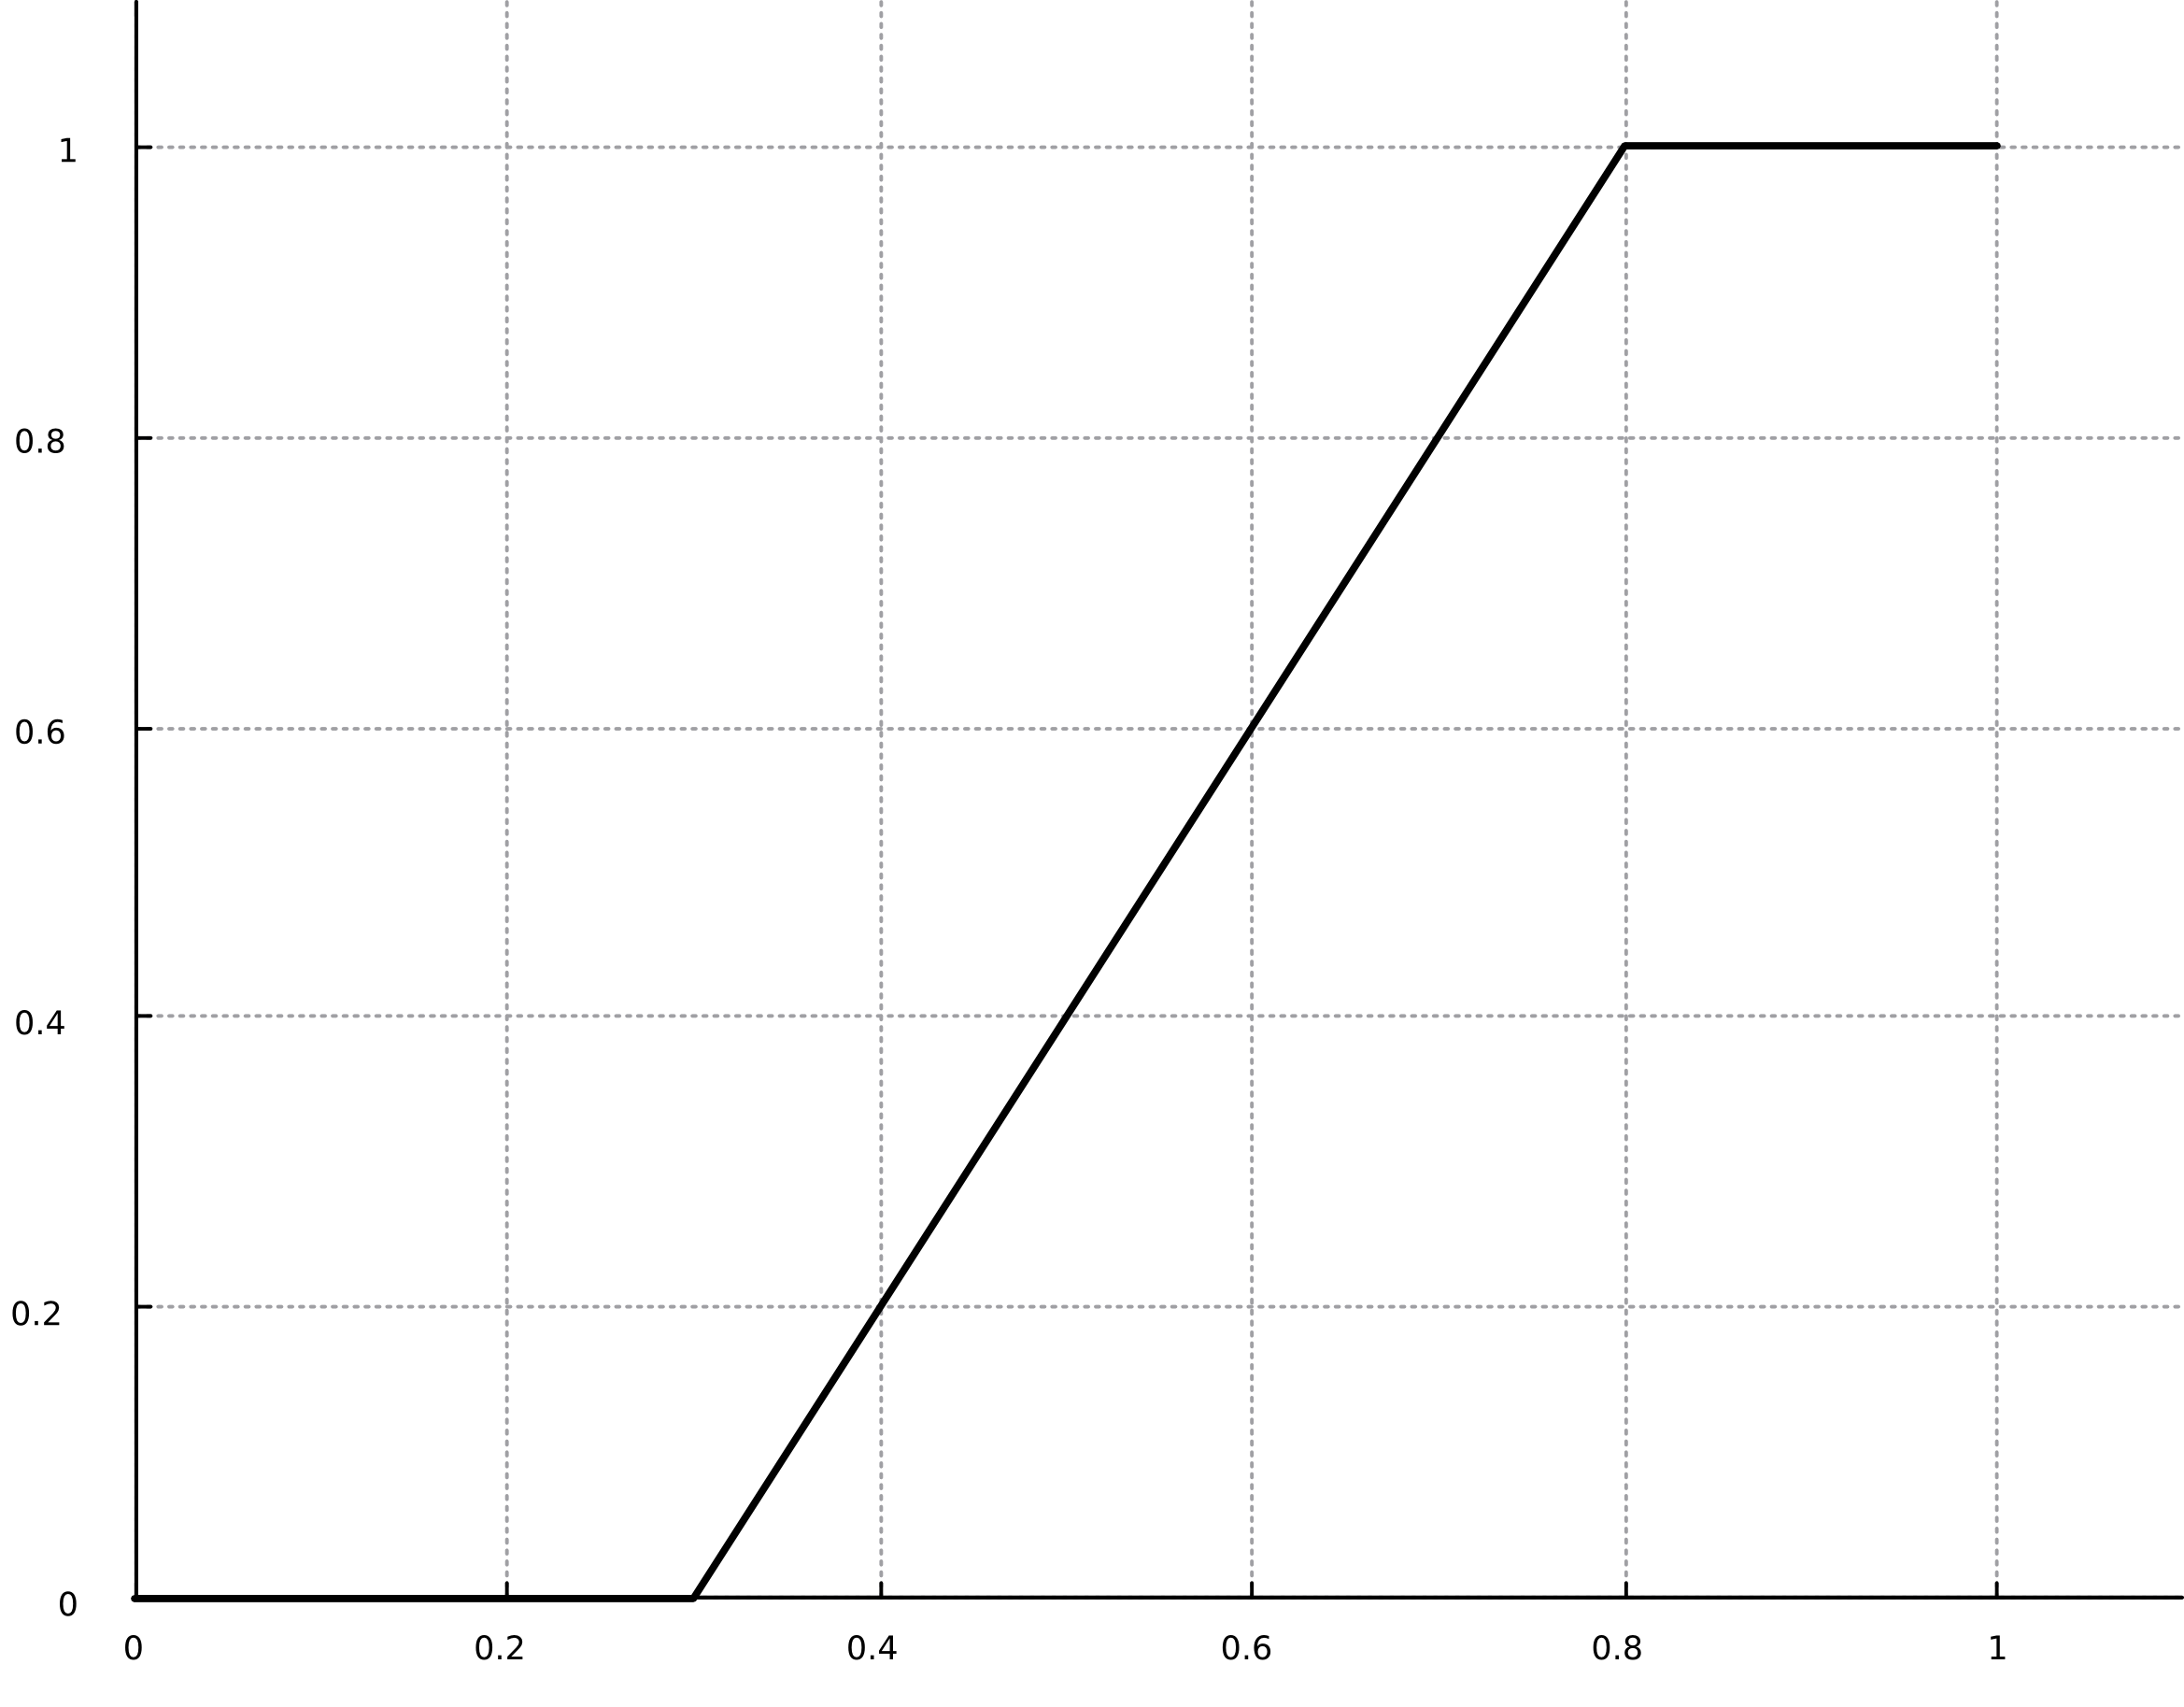
\includegraphics[width=\linewidth]
  	{chapters/fuzzylogic/fuzzy_most}
  \caption{Kwantyfikator lingwistyczny ,,Większość''}
  \label{fig:kwantyfikator_lingwistyczny_wiekszosc}
\end{figure}

\begin{figure}[ht]
  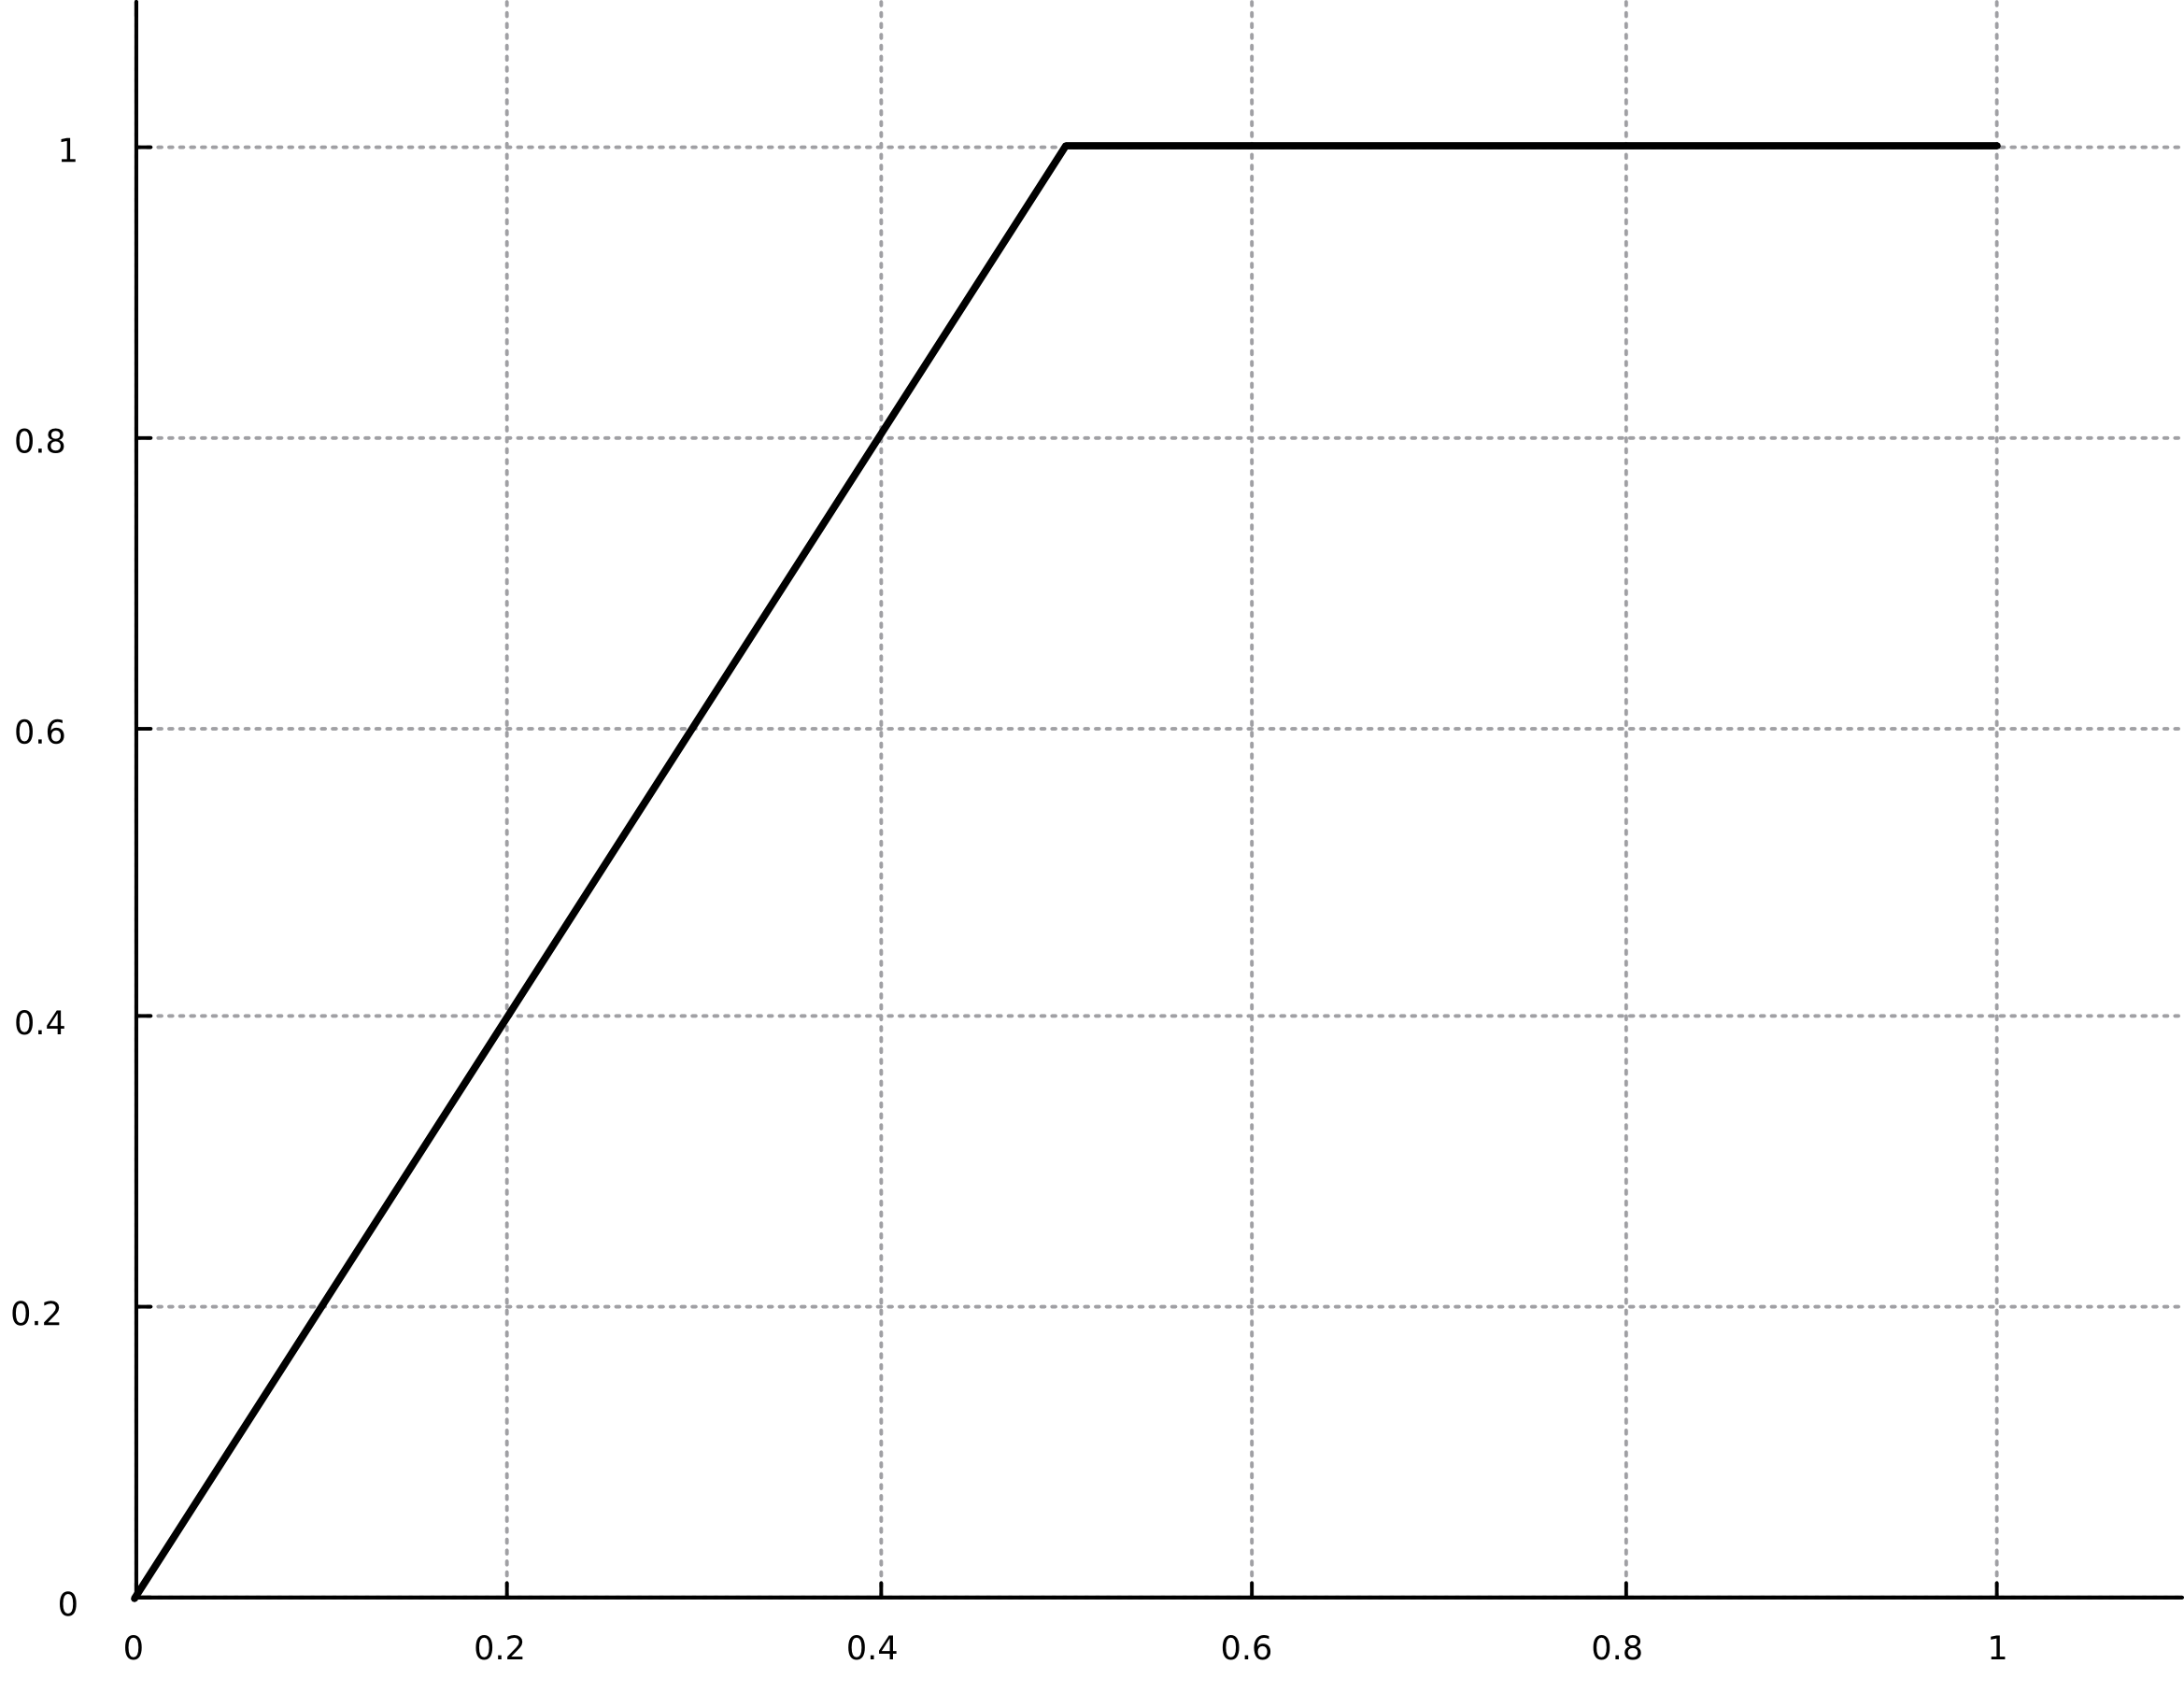
\includegraphics[width=\linewidth]
  	{chapters/fuzzylogic/fuzzy_half}
  \caption{Kwantyfikator lingwistyczny ,,Co najmniej połowa''}
  \label{fig:kwantyfikator_lingwistyczny_polowa}
\end{figure}

\begin{example}
Załóżmy, że stopnie preferencji każdego z ekspertów dla alternatywy $a$
wyglądają następująco: $[0.58, 0.33, 0.92, 0.08, 0.72, 0.65]$, a do agregacji
został użyty kwantyfikator lingwistyczny $Q = \textrm{,,większość''}$. Stopień
dominacji grupowej wynosi:
$$e(a) = F_{Q_{Most}}(0.58, 0.33, 0.92, 0.08, 0.72, 0.65) = 0.613,$$
gdzie $w=(0, 0.07, 0.33, 0.60, 0, 0).$
\end{example}

Z powyższego przykładu wynika, że kwantyfikator lingwistyczny ,,Większość''
bierze środkową część uporządkowanych ocen ekspertów i oblicza ich sumę ważoną.
Z powodzeniem można skorzystać z innych kwantyfikatorów, odpowiednio do
sytuacji. Ponadto przy pomocy operatora OWA można modelować sytuację, w której
decydenci zamierzają oceniać tak, że ,,większość'' kryteriów jest spełniona.

\section{Zastosowanie logiki rozmytej w podejmowaniu decyzji}
Podejmowanie decyzji to proces analizy zaistniałej sytuacji, z której istnieją 
co najmniej dwie drogi dalszego postępowania. Proces ten można oprzeć na 
racjonalnym działaniu, czyli logicznym myśleniu i chłodnej kalkulacji. Niestety 
w życiu codziennym wiele decyzji podejmowanych jest z wykorzystaniem własnych 
odczuć, emocji, intuicji. Zatem podejmowanie decyzji to proces nie tylko 
racjonalny i nowoczesne systemy wspomagania decyzji wprowadzają mechanizmy 
pozwalające na ocenę intuicyjną oraz działaniu na niepewnych i niepełnych 
danych.

Człowiek z natury porusza się w środowisku nieprecyzyjnym. Każdy potrafi 
powiedzieć, czy w danej restauracji smakuje mu jedzenie (wyśmienite, smaczne,
przeciętne, niesmaczne, $\dotsc$). Jednak mało kto potrafi w sposób ścisły, z
użyciem liczb, sprecyzować swoją opinię. Jest to subiektywna sprawa, osobiste
odczucie. Nieprecyzyjność jest całkowicie naturalna i stanowi nieodłączny
element podejmowania decyzji.

Grupowe podejmowanie decyzji jest bardzo dobrym przykładem na to, że 
modelowanie tego procesu tylko przy użyciu metod precyzyjnych jest zadaniem 
bardzo trudnym, a co więcej - nienaturalnym.

Poniższy podrozdział prezentuje przykłady wykorzystania logiki rozmytej w 
modelowaniu poszczególnych etapów grupowego podejmowania decyzji.

\subsection{Reprezentacja preferencji}
Każdy z decydentów powinien wyrazić swoją opinię na temat dostępnych alternatyw 
w sposób wygodny i naturalny, możliwie jak najbardziej zbliżony do naturalnego. 
Większość ludzi zapytanych o porównanie dwóch rozwiązań, jako pierwsze powie, 
że rozwiązanie pierwsze woli bardziej niż drugie. Może też paść odpowiedź ,,dużo
bardziej'', ,,zdecydowanie'' i tym podobne. Tego typu przypadki bardzo dobrze
modeluje powszechnie stosowana tak zwana rozmyta relacja preferencji.

Żeby w pełni wykorzystać możliwości rozmytej relacji preferencji, wykorzystuje 
się zmienną lingwistyczną. To dzięki niej możliwe jest wykorzystanie w 
obliczeniach wyrażeń lingwistycznych takich jak ,,mniej'' i ,,bardziej''.

Rozmytym oraz tradycyjnym metodom wydobywania i reprezentacji preferencji 
decydentów poświęcony został osobny rozdział.

\subsection{Ocena globalna}
Zazwyczaj na początku wszyscy członkowie grupy posiadają odmienne zdanie na 
temat wyboru rozwiązania. Proces osiągania konsensusu jest niezbędny w każdym 
procesie grupowego podejmowania decyzji. Tradycyjnie konsensus jest postrzegany 
jako pełna zgoda wszystkich decydentów. Oczywiście, ten typ konsensusu jest 
idealny i bardzo trudny do osiągnięcia. Z tego względu, jest to proces 
dynamiczny i iteracyjny. W jakiś sposób należy sprawdzać, czy odpowiedni poziom 
zgody został osiągnięty. Realizuje się to poprzez obliczenie globalnej oceny 
alternatyw i porównanie jej z indywidualnymi.

We wcześniejszym podpunkcie zostały przedstawione zbiory rozmyte jako doskonałe
narzędzie do reprezentacji ocen poszczególnych decydentów. Jest to również
doskonałe narzędzie do agregacji tych ocen w jedną zbiorczą ocenę. W tym celu
wykorzystuje się operatory agregacji, szczególnie operator OWA. Dzięki niemu
można mówić o konsensusie ,,większości'' albo ,,więcej niż $70\%$''
grupy.

\subsection{Tworzenie rankingu}
Po fazie agregacji następuje faza eksploatacji uzyskanych danych, czyli moment,
w którym ocena globalna alternatyw zamieniana jest na globalny ranking. Globalny
ranking uzyskuje się poprzez użycie dwóch stopni wyboru alternatyw:
kwantyfikator stopnia dominacji (QGDD, ang. quantifier guided dominance degree)
oraz kwantyfikator stopnia nie-dominacji (QGNDD, ang. quantifier guided non
dominance degree). Pierwszy z nich jest używany, aby uzyskać przewagę jaką
posiada dana alternatywa nad pozostałymi w kontekście rozmytej większości. Drugi
kwantyfikator natomiast, podaje stopień w jakim każda z alternatyw nie jest
zdominowana przez rozmytą większość zbioru alternatyw. Sposób w jaki należy
połączyć te dwie informacje w celu uzyskania rankingu jest opisany w kolejnych
rozdziałach.
